\documentclass[12pt,a4paper]{article}
\usepackage[utf8]{inputenc}
\usepackage{amsmath}
\usepackage{geometry}
\usepackage{listings}
\usepackage{booktabs}
\usepackage{float}
\usepackage{graphicx}

\geometry{margin=2.5cm}

\lstset{
    basicstyle=\ttfamily\small,
    numbers=left,
    breaklines=true,
    frame=single,
    language=Python,
    tabsize=4
}

\title{\textbf{Report 1: Gradient Descent} \\ \large Deep Learning Project 1}
\author{Duong Tan Binh - 2540007}
\date{\today}

\begin{document}

\maketitle
\tableofcontents
\newpage

\section{Introduction}

Gradient descent is an iterative algorithm to find the minimum value of a function. The idea is to use the derivative to find the minimum value of $f(x)$, following these steps:
\begin{enumerate}
    \item Random initialization: $x = x_0$
    \item Assign: $x = x - r \cdot f'(x)$
    \item Re-compute $f(x)$. Stop if $f(x)$ is small enough, or repeat step 2 if not (can be many times!)
\end{enumerate}
Where $r \geq 0$ is called the \textit{learning rate}.

\section{Algorithm Description}

\subsection{Numerical Gradient}

I approximate the first-order derivative using the central-difference formula:
\[
    f'(x) \approx \frac{f(x + h) - f(x - h)}{2h}
\]
where $h$ is a small step size (default $h = 10^{-3}$).

\subsection{Update Rule}

Starting from an initial point $x_0$, each iteration updates the estimate by:
\[
    x_{t+1} = x_t - r \cdot f'(x_t)
\]
The algorithm terminates when the absolute gradient falls below a threshold $\epsilon$:
\[
    |f'(x_t)| < \epsilon
\]

\subsection{Implementation}

\begin{lstlisting}[caption={Gradient Descent Implementation}]
def grad(f, x, h=1e-3):
    return (f(x + h) - f(x - h)) / (2 * h)

def f_(f, x0, r=0.1, threshold=1e-6):
    x = x0
    step = 0
    while True:
        g = grad(f, x)
        x = x - r * g
        step += 1
        print(f"Time: {step} Current x: {x:.8f}, f(x): {f(x):.8f}, Gradient: {g:.8f}")
        if abs(g) < threshold:
            break
    return x

result = f_(lambda x: x**2, x0=10, r=0.1)
\end{lstlisting}

\section{Experiment: Minimizing $f(x) = x^2$}

Running the algorithm with $x_0 = 10$, $r = 0.1$, and threshold $10^{-6}$:

\begin{table}[H]
\centering
\caption{Gradient descent on $f(x)=x^2$, $r=0.1$, $x_0=10$}
\begin{tabular}{rrrr}
\toprule
\textbf{Time} & $x$ & $f(x)$ & Gradient \\
\midrule
1  & 8.00000000 & 64.00000000 & 20.00000000 \\
2  & 6.40000000 & 40.96000000 & 16.00000000 \\
3  & 5.12000000 & 26.21440000 & 12.80000000 \\
5  & 3.27680000 & 10.73741824 &  8.19200000 \\
10 & 1.07374182 &  1.15292150 &  2.68435456 \\
20 & 0.11529215 &  0.01329228 &  0.28823038 \\
30 & 0.01237940 &  0.00015325 &  0.03094850 \\
40 & 0.00132923 &  0.00000177 &  0.00332307 \\
50 & 0.00014272 &  0.00000002 &  0.00035681 \\
60 & 0.00001532 &  0.00000000 &  0.00003831 \\
70 & 0.00000165 &  0.00000000 &  0.00000411 \\
77 & 0.00000035 &  0.00000000 &  0.00000086 \\
\bottomrule
\end{tabular}
\end{table}

The algorithm converged after 77 iterations, reaching $x \approx 3.5 \times 10^{-7} \approx 0$.
Both $x$ and $f(x)$ decrease monotonically toward $0$ at each step, confirming correct behavior.

\section{Effect of Different Learning Rate $r$}

The learning rate $r$ controls how large each update step is. To analyze its effect,
I ran \texttt{f\_plot()} on $f(x) = x^2$ with $x_0 = 10$ for four values of $r$
and plotted the gradient at each iteration.

\begin{table}[H]
\centering
\caption{Number of iterations to converge for different learning rates, $x_0 = 10$}
\begin{tabular}{ccc}
\toprule
\textbf{Learning Rate $r$} & \textbf{Iterations} & \textbf{Behavior} \\
\midrule
0.01 & 834 & Too slow, barely moves \\
0.1  & 77  & Smooth convergence \\
0.5  & 2   & Very fast (optimal for $x^2$) \\
0.9  & 77  & Oscillates but converges \\
\bottomrule
\end{tabular}
\end{table}

The figures below show the gradient value over iterations for each learning rate.

\begin{figure}[H]
\centering
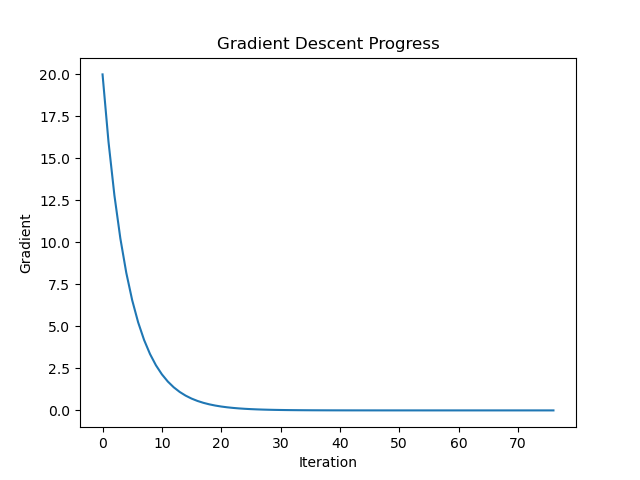
\includegraphics[width=0.7\textwidth]{gradient_descent_progress_01.png}
\caption{$r = 0.1$: smooth convergence in 77 iterations}
\end{figure}

\begin{figure}[H]
\centering
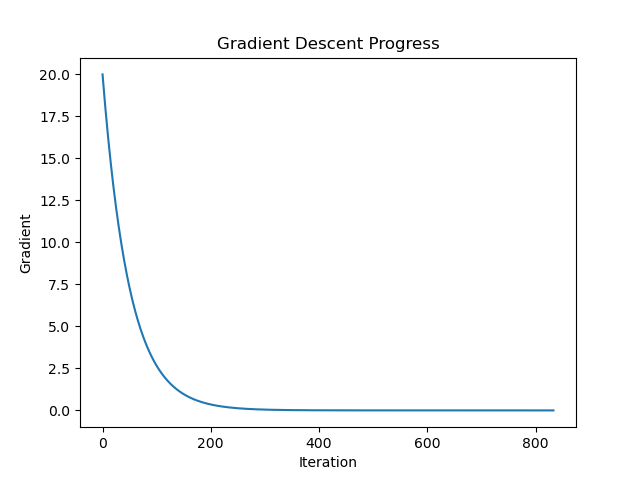
\includegraphics[width=0.7\textwidth]{gradient_descent_progress_001.png}
\caption{$r = 0.01$: very slow convergence, requires 834 iterations}
\end{figure}

\begin{figure}[H]
\centering
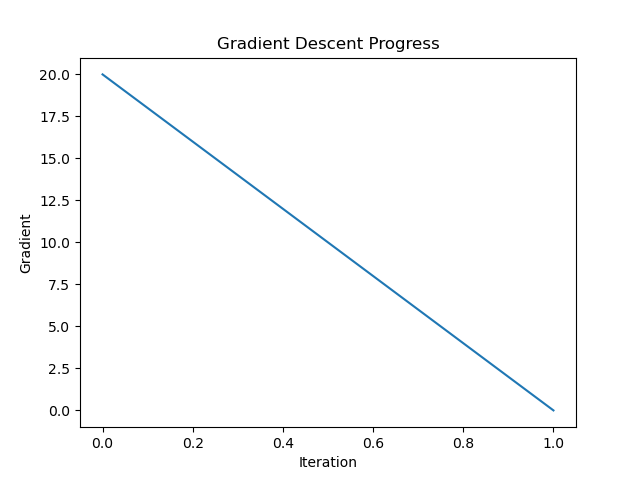
\includegraphics[width=0.7\textwidth]{gradient_descent_progress_05.png}
\caption{$r = 0.5$: converges in just 2 iterations (optimal for $x^2$)}
\end{figure}

\begin{figure}[H]
\centering
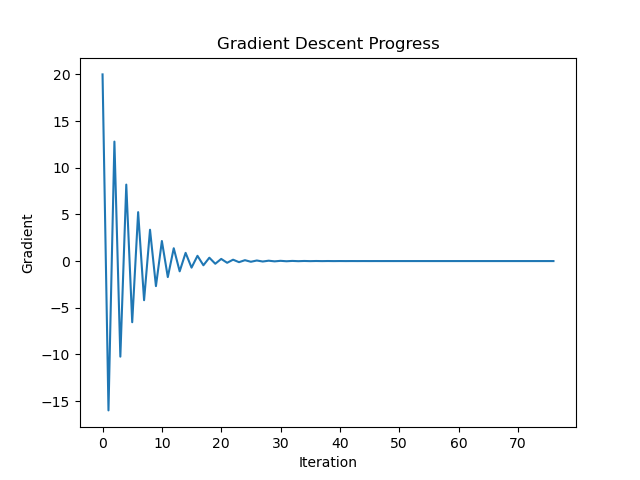
\includegraphics[width=0.7\textwidth]{gradient_descent_progress_09.png}
\caption{$r = 0.9$: oscillates before converging in 77 iterations}
\end{figure}

\section{Conclusion}

I implemented gradient descent from scratch using a central-difference numerical gradient.
The algorithm correctly converges to the minimum $x^* = 0$ of $f(x) = x^2$,
with $x$ and $f(x)$ decreasing monotonically toward zero at each iteration.

\end{document}